Existen tres categorías diferentes de conectores:


\begin{itemize}
\item \textbf{Simplex}, conector con una fibra terminada
\item \textbf{Dúplex}, conector con dos fibras terminadas
\item \textbf{Multifibra}, conector con más de dos fibras (hasta 72)
\end{itemize}


Los conectores simplex son actualmente los más frecuentes para despliegues FTTH. La figura~\figref{fig:Simplex_connectors} muestra los tipos más comunes de conectores simplex:


\begin{figure}[H]
	\centering
	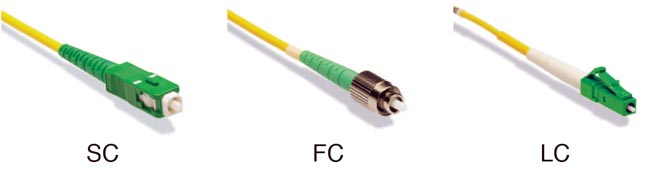
\includegraphics[width=0.80\textwidth]{./img/punto6/Tipos-de-conectores-simplex.jpg}
	\caption{Tipos de conectores simplex}
	\label{fig:Simplex_connectors}
\end{figure}


Otra categoría de conector utilización creciente es el conector multifibra (o MT). Un conector MT individual puede tener desde 4 a 72 fibras. El tipo de conector multifibra utilizado de forma más generalizada en PONs es el tipo MTP. Este conector es utilizado frecuentemente para la confección de latiguillos múltiples de expansión, de especial utilidad en instalaciones de gran densidad de fibras.


\begin{wrapfigure}[10]{l}{0.55\textwidth}
  \begin{center}
   	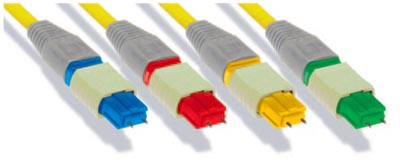
\includegraphics[width=0.55\textwidth]{./img/punto6/Conector-MTP.jpg}	
   	\caption{Conector MTP (fuente US Conec)}
	\label{fig:MTP_connector}
  \end{center}  
\end{wrapfigure}

Cabe indicar, no obstante, que el tipo de conector más frecuente en implantaciones FTTH, por el momento, es el conector de pulido en ángulo (APC), principalmente debido a que la inclinación de 8º en la ferrule proporciona pérdidas de reflexión superiores 60 dB (la pérdida de inserción típica es ≤ 0,5 dB). Los conectores APC pueden identificarse de forma sencilla por su color verde (ver figura~\figref{fig:MTP_connector}).









